\section{Vivado仿真验证}

\subsection{仿真环境配置}

% TODO: 描述仿真testbench的设置，包括时钟周期、复位信号等

使用Vivado自带的仿真工具（Vivado Simulator）对CPU设计进行功能仿真。仿真顶层模块为 \texttt{openmips\_min\_sopc\_tb}，主要配置如下：

\begin{itemize}[leftmargin=2em]
    \item 仿真时钟周期：20ns（50MHz）
    \item 复位信号：仿真开始时拉高，经过若干个时钟周期后释放
    \item 仿真时长：根据测试程序执行所需周期数设定
\end{itemize}

\subsection{仿真波形分析}

% TODO: 插入Vivado仿真波形截图，并对关键信号进行分析

\begin{figure}[H]
    \centering
    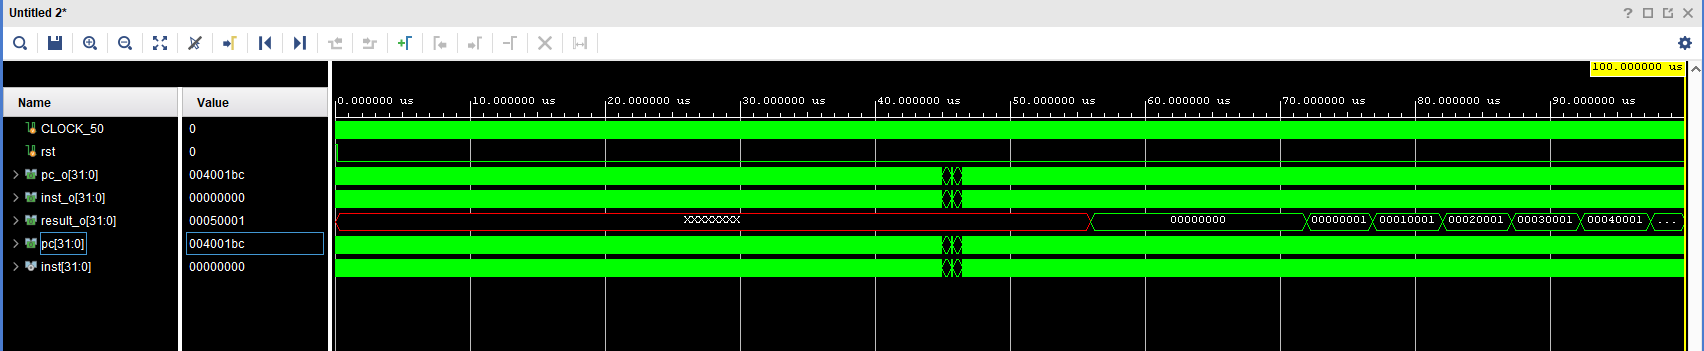
\includegraphics[width=0.9\textwidth]{img/sim_waveform1.png} 
    \caption{仿真波形——整体执行过程}
\end{figure}


\subsection{仿真结果}


